\pagebreak

\section*{Problema 06}

\textbf{Compute the gradient $\nabla (x)$ and Hessian $\nabla^2 f (x)$ of the Rosenbrock function}

\begin{equation*}
    f(x) = \sum_{i=1}^{N-1}[100(x_{i+1}-x_i^2)+(1-x_i)^2]
\end{equation*}

\textbf{where $x = [x_1 ,\dots, x_N ]^T \in R^N$ If n = 2 show that $x^*  = [1, 1]^T$ is the only local minimizer of this function, and that the Hessian matrix at that point is positive definite. Plot the contour lines of f.}

Para $n=2$ se obtiene que $f(x)$ es:

\begin{equation*}
    f(x) = 100(x2-x_1^2)^2 +(1-x_1)^2
\end{equation*}

Calculando el gradiente se obtiene lo siguiente:

\begin{equation*}
    \dpartial{f(x)}{x_1} = -400(x_2-x_1^2)x_1 -2(1-x_1)x_1
\end{equation*}

\begin{equation*}
    \dpartial{f(x)}{x_2} = 200(x_2-x_1^2)
\end{equation*}

A partir de $\partial_{x_2} f(x)=0$, se obtiene la realcion $x_2=x_1^2$. Usando esta relación en $\partial_{x_1}f(x)$ se obtiene que $x_1=0,1$, por ende $x_2=0,1$. Dando así, los puntos críticos de $f(x)$ son $\{(0,0),(1,1)\}$.

Calculando el hessiano de $f(x)$ se obtiene que:

\begin{equation*}
    \dpartial{^2f(x)}{x_1^2} = 800x_1^2 -400(x_2-x_1^2)+2x-2(1-x_1)
\end{equation*}

\begin{equation*}
    \dpartial{^2f(x)}{x_2^2} = 200
\end{equation*}

\begin{equation*}
    \dpartial{^2f(x)}{x_2x_1} = -400x_1
\end{equation*}

Por lo tanto, el hessiano es:

\begin{equation*}
    \nabla^2f(x) = \begin{bmatrix}
        800x_1^2 -400(x_2-x_1^2)+2x-2(1-x_1) & -400x_1 \\
        -400x_1                              & 200
    \end{bmatrix}
\end{equation*}

Evaluando en $(0,0)$ se obtiene que $|\nabla^2 f(0,0)|=-400$, por lo que ese punto representa un punto silla. En cambio evaluando se obtiene que $|\nabla^2 f(1,1)|=400$ y $\partial^2_{x_1}f(1,1)=802$. Por lo que este representa un punto mínimo.

En la figura \ref{fig:problem_6} se representa las curvas de nivel de la función $f(x)$.

\begin{figure}[H]
    \centering
    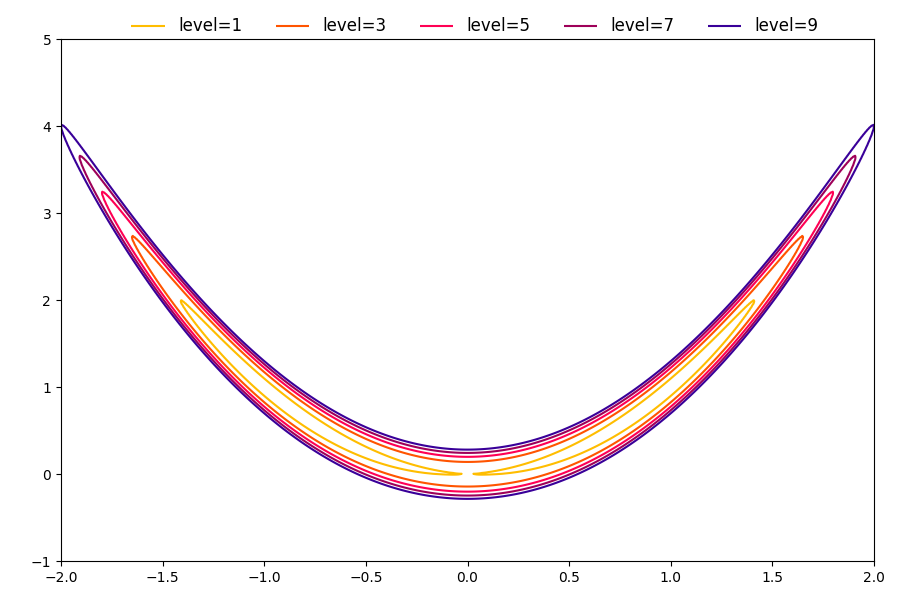
\includegraphics[width=12cm]{Graphics/problem06.png}
    \caption{Curvas de niel de la función $f(x)$.}
    \label{fig:problem_6}
\end{figure}